\documentclass[12pt,letterpaper]{article}

\usepackage[top=1.80cm,left=1.90cm,right=1.90cm,bottom=1.7cm,includeheadfoot]{geometry}

\setlength{\headheight}{27.52466pt}
\setlength{\footskip}{22pt}
\setlength{\headsep}{8pt}
%\setlength{\parskip}{0.5ex}

\usepackage[protrusion=true,expansion=true]{microtype}
\usepackage[T1]{fontenc}

%\usepackage[bitstream-charter]{mathdesign} % Charter BT

\usepackage{times}                        % Times New Roman

%\usepackage{palatino,mathpazo}            % Palatino
\RequirePackage[scaled=0.92]{helvet}
%\RequirePackage[scaled=1.02]{inconsolata}
%\linespread{1.05}

\usepackage{fancyhdr}
\pagestyle{fancy}
\chead{\textbf{\sffamily Research Proposal}\\
\sffamily Title of the Grant Goes Here}
\lhead{\sffamily Lastname, Firstname I.\\}
\rhead{\sffamily Amount requested: \$xxx,xxx\\}
\cfoot{\small\sffamily Research Proposal Page \thepage}
\renewcommand{\headrulewidth}{0.4pt}% default is 0pt
\renewcommand{\footrulewidth}{0.4pt}% default is 0pt

\usepackage{graphicx}
\usepackage[labelfont=bf,skip=3ex,width=0.9\textwidth]{caption}

\usepackage{citecollapse}
\usepackage[nospace]{cite}

\let\oldthebibliography=\thebibliography
\let\endoldthebibliography=\endthebibliography
\renewenvironment{thebibliography}[1]{%
  \begin{oldthebibliography}{#1}%
    \setlength{\parskip}{0ex}%
    \setlength{\itemsep}{0.25ex}%
}%
{%
  \end{oldthebibliography}%
}

\usepackage[compact]{titlesec}
\titlespacing*{\section}{0pt}{0.75ex}{0.25ex}
\titleformat*{\section}{\centering\normalsize\bfseries\sffamily}
\titlespacing*{\subsection}{0pt}{1.0ex}{0pt}
\titlespacing*{\subsection}{0pt}{0.75ex}{0.25ex}
\titleformat*{\subsection}{\normalsize\bfseries\sffamily}
\titlespacing*{\subsubsection}{0pt}{0.75ex}{0.25ex}
\titleformat*{\subsubsection}{\normalsize\bfseries\sffamily}

\usepackage{lipsum}

\begin{document}

\section*{Background}

In Figure~\ref{fig:brain} you can see a picture of a brain. Here are two citations to some papers \cite{HODGKIN:1952aa,HODGKIN:1952ab,Hodgkin:1947aa} and another \cite{Hodgkin:1990aa}. Quisque ullamcorper placerat ipsum. Cras nibh. Morbi vel justo vitae lacus tincidunt ultrices. Lorem ipsum dolor sit amet, consectetuer adipiscing elit. In hac habitasse platea dictumst.

\lipsum[1-9]


\section*{Project 1}

\lipsum[1-2]

\subsection*{Experiment 1.1}

\lipsum[1-5]

\subsection*{1.1 Pilot Data}

\lipsum[1-2]


\section*{Significance}

\lipsum[1-2]

\newpage
\onecolumn
\bibliography{refs}
\bibliographystyle{cihr} % created cihr.bst with "latex makebst" command


\newpage
\clearpage
\begin{figure}[H]
  \centering
  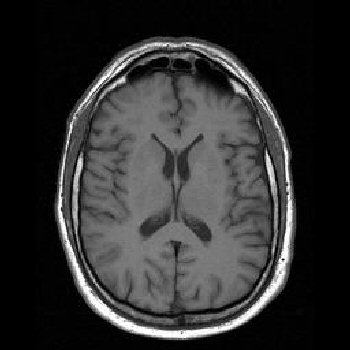
\includegraphics[width=4in]{figures/t1_brain.jpg}
  \caption{This is a picture of a brain.}
  \label{fig:brain}
\end{figure}


\end{document}

 


